\chapter{Evaluation}
\label{sec:Evaluation}

\section{Test Environment}
For the purpose of evaluation, the crill cluster at the Research and Computing Center of the University of Houston was used.

\subsection{Crill Cluster Hardware Specification}
\begin{itemize}
\item \textbf{16 NLE Systems nodes (crill-001 - crill-016)}\\
  Four 2.2 GHz 12-core AMD Opteron processors (48 cores total)\\
  64 GB main memory\\
  Two dual-port 4xDDR InfiniBand HCAs

\item \textbf{2 Appro 1326G4 nodes (crill-101 - crill-102)}\\
  Two 2.2 GHz 12-core AMD Opteron processors (24 cores total)\\
  32 GB main memory\\
  Four NVIDIA Tesla M2050 GPUs (448 cores each)\\
  4xDDR InfiniBand HCA

\item \textbf{4 HP DL 160 Gen 8 nodes (crill-200 - crill-203)}\\
  Two 2.4 GHz quad-core Intel Xeon E5-2665 processors (24 cores total)\\
  8 GB main memory\\
  4xDDR InfiniBand HCA
  
\item \textbf{Network Interconnect}\\
  144 port 4xInfiniBand DDR Voltaire Grid Director ISR 2012 switch (shared with whale cluster)\\
  24 port 4xInfiniBand SDR switch (I/O switch to the SSD storage)\\
  48 port Netgear GE switch

\item \textbf{Storage}\\
  2 TB RamSan 620 SSD storage (/pvfs2-ssd)\\
  20 TB Sun StorageTek 6140 array (/home shared with shark cluster)\\
  8 TB distributed PVFS2 storage (/pvfs2)
  
\end{itemize}

\subsection{Crill Cluster Nodes Software Specification}
\begin{itemize}
\item \textbf{Operating System}\\
  Linux kernel version 3.11.10-21-desktop\\
  Distribution: openSUSE 13.1 (x86\_64)
\item \textbf{Open MPI} version 1.8
\item \textbf{HPX} version 0.9.10 release
\item \textbf{Boost} version 1.55.0
\item \textbf{GCC and G++} version 4.8.1
\end{itemize}


\section{Configuration, Compilation, and Execution}

\subsection{Open MPI Configuration Parameteres}
For running different test cases, our evaluation is mostly focused on comparison between Open MPI using ORTE vs. Open MPI using HPX-RTE as runtime.
Listing \ref{lst:config-hpxrte} shows the configure line for the Open MPI installation. The only parameter that needs to be changed is \verb|--with-orte|. When this parameter is set to ``yes'', Open MPI uses ORTE as runtime. If we set this parameter to ``no'', Open MPI will use HPX-RTE.

\begin{lstlisting}[language=C, frame=single, basicstyle=\footnotesize, caption=Configure Line of Open MPI with HPX-RTE\label{lst:config-hpxrte}]
  $ ./configure CFLAGS=``-g -O0'' CXXFLAGS=``-g -O0''
    --prefix=/home/hadi/opt/openmpi
    --with-hpx=/opt/hpx-0.9.10-release
    --with-boost=/opt/boost/1-55-0
    --disable-vt --enable-mca-no-build=coll-ml,vprotocol
    --enable-oshmem=no --enable-mpi-profile=no
    --enable-static --with-orte=no
\end{lstlisting}

\subsection{Compiling MPI Applications}
Listing \ref{lst:compile} illustrates the compile line for our Hello World example. This line could be integrated into Open MPI software in future iterations of the development. Therefore, users will not have to manually insert all the compile and linkage flags needed. The same command can be used when ORTE is the installed runtime.

\begin{lstlisting}[language=C, frame=single, basicstyle=\footnotesize, caption=Compile Line for Hello World\label{lst:compile}]
  $ mpicxx -o mpi_hello mpi_hello.c -rdynamic -fPIC -std=c++11
  -Wall -Wno-unused-local-typedefs -Wno-strict-aliasing
  -Wsign-promo -Wno-cast-align -Werror=vla -Werror=return-type
  -fdiagnostics-show-option  -Werror=uninitialized -pthread
  -DHPX_DEBUG -D_GNU_SOURCE  -I${HPX_DIR}/include/hpx/external
  -I${HPX_DIR}/include -I/usr/include/google
  -DHPX_APPLICATION_EXPORTS -DHPX_ENABLE_ASSERT_HANDLER
  -DHPX_DEBUG -finline-functions -I/opt/boost/1-55-0/include
  -L/opt/boost/1-55-0/lib -Wl,-rpath,:${HPX_DIR}/lib/hpx
  -L${HPX_DIR}/lib/hpx -L${HPX_DIR}/lib -lhpx -lhpx_init
  -lhpx_serialization -lboost_date_time -lboost_filesystem
  -lboost_program_options -lboost_regex -lboost_serialization
  -lboost_system -lboost_thread -lboost_atomic -lboost_chrono
  -lprofiler -liostreams -L/lib64 -lrt -ldl -lutil -g -O0
\end{lstlisting}


\subsection{Running MPI Applications}
For running applications using ORTE, we will use ``mpirun'' command, which is a soft link to ``orterun'' command. This is shown in listing \ref{lst:orterun}. ORTE also supports a direct launch mechanism which avoids creating the ORTE daemons on individual compute nodes but uses the native resource manager instead for the management services, e.g. an application can be started directly using the srun command in a SLURM enviornment. This version has lower startup costs, but reduces the functionality of the runtime environment.

\begin{lstlisting}[language=C, frame=single, basicstyle=\footnotesize, caption=Running MPI Applications Using ORTE \label{lst:orterun}]
$ mpirun -np 1 -pernode ./mpi_hello
\end{lstlisting}

HPX provides support for Slurm (Simple linux utility for resource management)~\cite{yoo2003slurm}. To run applications using HPX-RTE, we use ``srun'' command. Listing \ref{lst:hpxrte-run} demonstrates an example.

\begin{lstlisting}[language=C, frame=single, basicstyle=\footnotesize, caption=Running MPI Applications Using HPX-RTE \label{lst:hpxrte-run}]
$ srun -N 1  -n 1 --ntasks-per-node=1 ./mpi_hello --hpx:run-hpx-main
  --hpx:threads=2
\end{lstlisting}


\section{Evaluation}
In our evaluations, there are two ways to measure the time in the case of each application: The total time measured by the ``time'' command in Linux, and measuring the time within the application. The time reported by the application is reported on a per process basis in some test cases. Numbers reported in this section are averge numbers reported by the application when the application reported times are reported. Every test was run at lesat three times. The average of all three times is reported.


\subsection{Parallel Computational Fluid Dynamics}
We use an MPI implementation~\cite{resch1999comparison} of a computational fluid dynamics (CFD) test case defined by Ecer, Satofuka, Periaux, and Taylor, 2006~\cite{ecer1996parallel}.
The objective is to solve the following partial differential equation (PDE) on a parallel computer:
\[
\frac{df}{f} = \Delta f
\]
This test case uses an explicit scheme with forward time and centered space. The equation is solved over a cube of unit dimensions. The initial conditions everywhere inside the cube are: f = 0. The boundary conditions are: f = x on all edges. The implementation calculates the steady-state solution.

Figure \ref{fig:time-all-heatsolver-100-infiniband} shows the time spent running the application using ORTE and HPX-RTE. Figure \ref{fig:time-app-heatsolver-100-infiniband} illustrates the times reported by the application using ORTE and HPX-RTE. We ran the application with different number of processes (1, 2, 4, 8, and 16). The grid dimensions are 100x100x100.

\begin{figure}[h!]
  \centering
  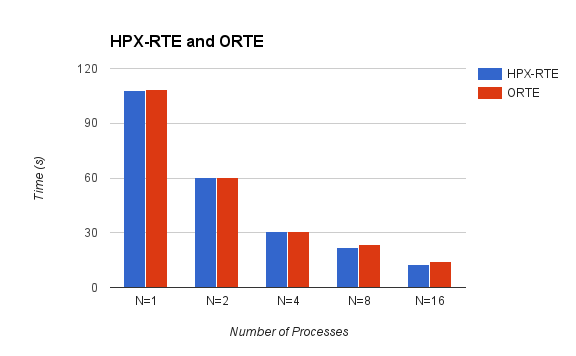
\includegraphics[scale=0.7]{images/time-all-heatsolver-100-infiniband.png}
  \caption[CFD Running Time - 100x100x100]{CFD Running Time - 100x100x100}
  \label{fig:time-all-heatsolver-100-infiniband}
\end{figure}

\begin{figure}[h!]
  \centering
  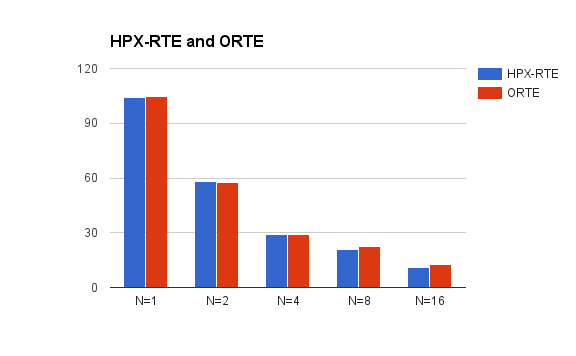
\includegraphics[scale=0.7]{images/time-app-heatsolver-100-infiniband.png}
  \caption[CFD Application Reported Time - 100x100x100]{CFD Application Reported Time - 100x100x100}
  \label{fig:time-app-heatsolver-100-infiniband}
\end{figure}

Both Figure \ref{fig:time-all-heatsolver-100-infiniband} and Figure \ref{fig:time-app-heatsolver-100-infiniband} demonstrate that despite slight better time performance using HPX-RTE in most cases, the overall times are very close. We believe this is because the overall time is dominated by communication and computation over the time spent by the runtime. To verify this, we decreased the problem size and used a grid of size 80x80x80. The results shown in Figure \ref{fig:time-all-heatsolver-80-infiniband} and Figure \ref{fig:time-app-heatsolver-80-infiniband} support this hypothesis. As we decrease the problem size, the time difference becomes more distinct.

\begin{figure}[h!]
  \centering
  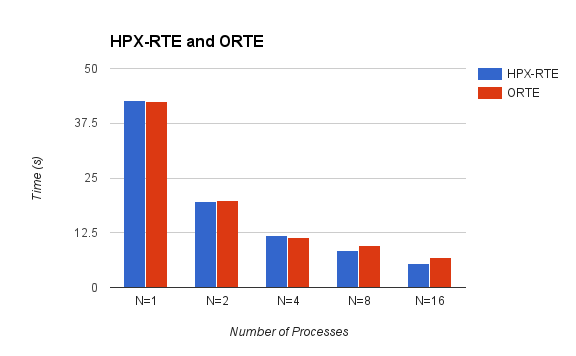
\includegraphics[scale=0.7]{images/time-all-heatsolver-80-infiniband.png}
  \caption[CFD Running Time - 80x80x80]{CFD Running Time - 80x80x80}
  \label{fig:time-all-heatsolver-80-infiniband}
\end{figure}

\begin{figure}[h]
  \centering
  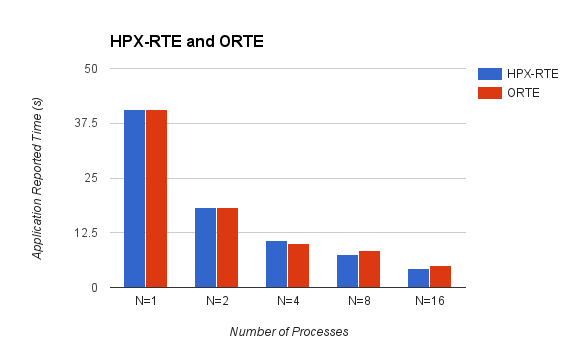
\includegraphics[scale=0.7]{images/time-app-heatsolver-80-infiniband.png}
  \caption[CFD Application Reported Time - 80x80x80]{CFD Application Reported Time - 80x80x80}
  \label{fig:time-app-heatsolver-80-infiniband}
\end{figure}

To better understand the effect of the runtime, we can study an example with minimal communication and computation. 

\clearpage
\subsection{MPI Hello World}
A very-good example to study the performance of the runtime would be a simple ``Hello World'' example (Listing \ref{lst:mpi_hello}). Since this simple application includes minimum communication and computation time, it could give us a better picture of the time spent in the runtime. Figure \ref{fig:time-all-hello-world-infiniband} illustrates the running time measured by the ``time'' command. Figure \ref{fig:time-app-hello-world-infiniband} shows the time measured starting before \verb|MPI_Init()| until after \verb|MPI_Finalize()| funtion. There is an improvement of up to \textbf{53\%} using HPX-RTE over ORTE.

\begin{lstlisting}[language=C, frame=single, basicstyle=\footnotesize, caption=MPI Hello World \label{lst:mpi_hello}]
#include <mpi.h>
#include <hpx/hpx_main.hpp>
int main (int argc, char** argv)
{
  int rank, size;
  double t1, t2;
  t1 = MPI_Wtime();
  MPI_Init (&argc, &argv);
  MPI_Comm_rank (MPI_COMM_WORLD, &rank);
  MPI_Comm_size (MPI_COMM_WORLD, &size);
  printf( ``Hello world from process %d of %d\n'', rank, size );
  MPI_Finalize();
  t2 = MPI_Wtime();
  printf(``%1.4f\n'', t2-t1);
  return 0;
}
\end{lstlisting}

\begin{figure}[h!]
\centering
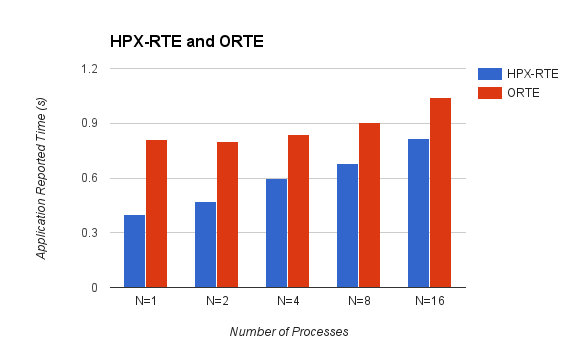
\includegraphics[scale=0.7]{images/time-all-hello-world-infiniband.png}
\caption[Time - Hello World]{Time - Hello World}
\label{fig:time-all-hello-world-infiniband}
\end{figure}

\begin{figure}[h!]
\centering
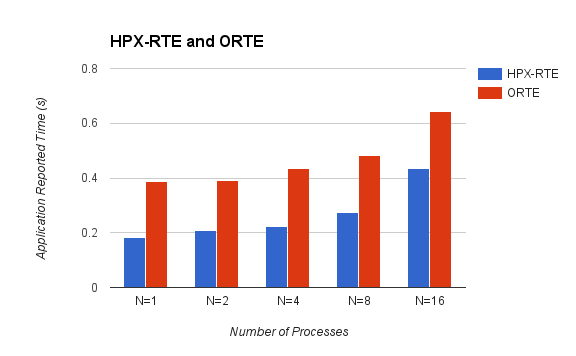
\includegraphics[scale=0.7]{images/time-app-hello-world-infiniband.png}
\caption[Application Reported Time - Hello World]{Application Reported Time - Hello World}
\label{fig:time-app-hello-world-infiniband}
\end{figure}

\clearpage
\subsection{Parallel Smoothing}
This application performs smoothing on an input image on a pixel-by-pixel basis. The algorithm changes the class that a pixel has been assigned to if majority of neighboring elements have a different class. For each pixel, we consider an area of 5x5 pixels (two pixels in each direction). Input file contains the integer value of the class that each pixel belongs to. The algorithm is performed iteratively 10 times, and the result is written to an output file.

Figure \ref{fig:time-all-smoother-1024-infiniband} and \ref{fig:time-app-smoother-1024-infiniband} show the running time and application reported time accordingly. The input image size is 1024x1024 pixels.

We can see a slight performance benefit using HPX-RTE in both cases. However, this is more obvious in the overal reported times. In the case of application reported time in this algorithm, the application is reporting only the smoothing part (communication and computation). The majority of the time spent in runtime (start up and shut down), reading from the input file, and writing to the output file are not inside the section of the code the application is reporting the time for. This shows that the computation and communication times are very close, and the actual difference comes from the choice of runtime. We ran the same test on an input image of size 2048x2048 pixels. The results are shown in Figure \ref{fig:time-all-smoother-2048-infiniband} and Figure \ref{fig:time-app-smoother-2048-infiniband}.

The comparison between two different input sizes shows that by increasing the problem size, the different between two runtimes becomes smaller and smaller. This is in accordance with what we suggested previously that the HPX-RTE runtime by itself is faster than ORTE, but the difference shows itself when the application is not dominated by communicational and computational work load.

\begin{figure}[h!]
  \centering
  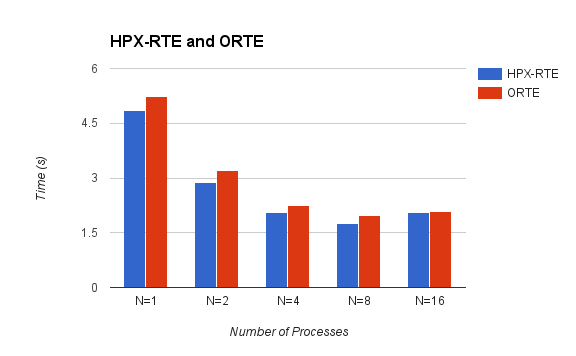
\includegraphics[scale=0.7]{images/time-all-smoother-1024-infiniband.png}
  \caption[Time - Parallel Smoothing - 1024x1024]{Time - Parallel Smoothing - 1024x1024}
  \label{fig:time-all-smoother-1024-infiniband}
\end{figure}

\begin{figure}[h!]
  \centering
  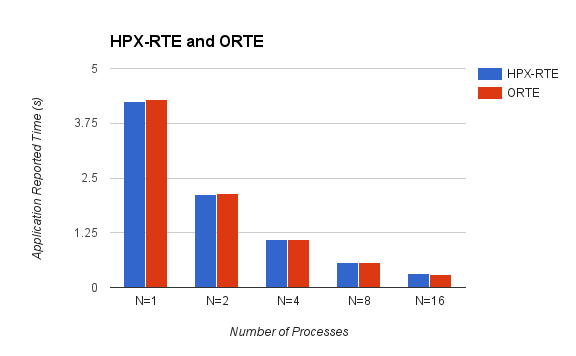
\includegraphics[scale=0.7]{images/time-app-smoother-1024-infiniband.png}
  \caption[Application Reported Time - Parallel Smoothing - 1024x1024]{Application Reported Time - Parallel Smoothing - 1024x1024}
  \label{fig:time-app-smoother-1024-infiniband}
\end{figure}


\begin{figure}[h!]
  \centering
  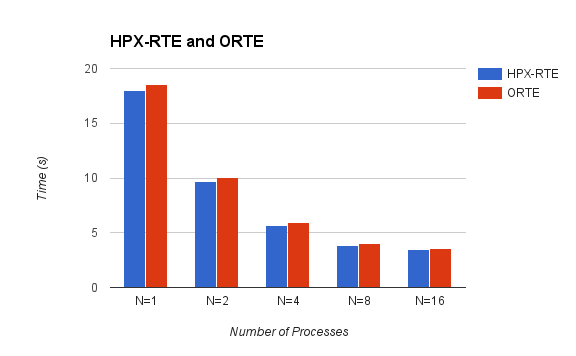
\includegraphics[scale=0.7]{images/time-all-smoother-2048-infiniband.png}
  \caption[Time - Parallel Smoothing - 2048x2048]{Time - Parallel Smoothing - 2048x2048}
  \label{fig:time-all-smoother-2048-infiniband}
\end{figure}

\begin{figure}[h!]
  \centering
  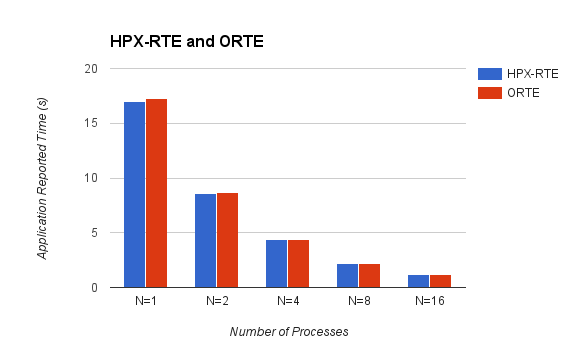
\includegraphics[scale=0.7]{images/time-app-smoother-2048-infiniband.png}
  \caption[Application Reported Time - Parallel Smoothing - 2048x2048]{Application Reported Time - Parallel Smoothing - 2048x2048}
  \label{fig:time-app-smoother-2048-infiniband}
\end{figure}


\clearpage
\subsection{Code Size}
Figure \ref{fig:code-size} shows a comparison between HPX-RTE and ORTE code size (number of lines of code).

\begin{figure}[h!]
  \centering
  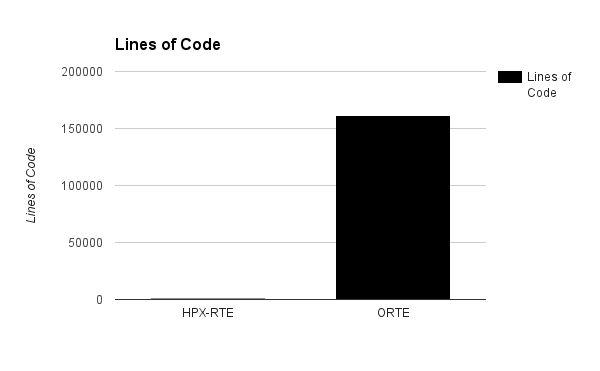
\includegraphics[scale=0.7]{images/code-size.png}
  \caption[Code Size Comparison - HPX-RTE and ORTE]{Code Size Comparison - HPX-RTE and ORTE}
  \label{fig:code-size}
\end{figure}

As it is shown in Figure \ref{fig:code-size}, the source code size for HPX-RTE is less than \textbf{0.64\%} of the code base for ORTE. This is partly because HPX-RTE is taking advantage of the HPX library and HPX-RTE component does not currently provide support for a number of features such as failure handling and dynamic process management that are supported by ORTE. Our evaluations in previous sections showed significant runtime performance improvement and very close overall performance using HPX-RTE over ORTE. Achieveing this level of performance with reducing the code size of the runtime by more than \textbf{99.36\%} is a significant improvement.

